%==============================================================================
% Sjabloon onderzoeksvoorstel bachproef
%==============================================================================
% Gebaseerd op document class `hogent-article'
% zie <https://github.com/HoGentTIN/latex-hogent-article>

% Voor een voorstel in het Engels: voeg de documentclass-optie [english] toe.
% Let op: kan enkel na toestemming van de bachelorproefcoördinator!
\documentclass{hogent-article}

% Invoegen bibliografiebestand
\addbibresource{voorstel.bib}
\usepackage{pdfpages}

% Informatie over de opleiding, het vak en soort opdracht
\studyprogramme{Professionele bachelor toegepaste informatica}
\course{Bachelorproef}
\assignmenttype{Onderzoeksvoorstel}
% Voor een voorstel in het Engels, haal de volgende 3 regels uit commentaar
% \studyprogramme{Bachelor of applied information technology}
% \course{Bachelor thesis}
% \assignmenttype{Research proposal}

\academicyear{2024-2025} % TODO: pas het academiejaar aan

% TODO: Werktitel
\title{De ideale CMS-oplossing: Een balans tussen kosten, gebruiksgemak en prestaties voor nagelsalons}

% TODO: Studentnaam en emailadres invullen
\author{Bente De Wilde}
\email{bente.dewilde@student.hogent.be}

% TODO: Geef de co-promotor op
\supervisor[Co-promotor]{S. Mesanovic (Sabi Nails)}

% Binnen welke specialisatierichting uit 3TI situeert dit onderzoek zich?
% Kies uit deze lijst:
%
% - Mobile \& Enterprise development
% - AI \& Data Engineering
% - Functional \& Business Analysis
% - System \& Network Administrator
% - Mainframe Expert
% - Als het onderzoek niet past binnen een van deze domeinen specifieer je deze
%   zelf
%
\specialisation{Mobile \& Enterprise development}
\keywords{Content Management System (CMS), Website optimalisatie, Gebruiksvriendelijkheid}

\begin{document}

\begin{abstract}
    In de huidige digitale wereld is een professionele online aanwezigheid essentieel voor bedrijven van elke omvang, maar het kiezen van een geschikt Content Management Systeem (CMS) kan uitdagend zijn, vooral voor kleine ondernemingen met beperkte middelen en technische kennis. Dit onderzoek richt zich op het vinden van de meest geschikte CMS-oplossing voor een nagelsalon, met specifieke aandacht voor gebruiksvriendelijkheid, kosten, prestaties en veiligheid.
    
    Door middel van interviews met de eigenaar van het nagelsalon worden de unieke behoeften en vereisten van dit type onderneming vastgesteld. Vervolgens wordt een vergelijkende analyse uitgevoerd van drie veelgebruikte CMS’en: WordPress, Joomla en Drupal. Op basis van vooraf gedefinieerde criteria worden proof-of-concepts (PoC’s) ontwikkeld en getest door de eigenaar om de praktische toepasbaarheid en gebruiksvriendelijkheid van elk systeem te beoordelen.
    
    De resultaten tonen aan dat WordPress het beste scoort op gebruiksvriendelijkheid en kostenbeheersing, waardoor het de meest geschikte keuze lijkt voor een nagelsalon met beperkte technische expertise. Dit onderzoek biedt een concrete aanbeveling en een demonstratie van de aanbevolen oplossing, waarmee de eigenaar van het nagelsalon een goed geïnformeerde keuze kan maken en kan profiteren van een eenvoudige, veilige en functionele website.
\end{abstract}

\tableofcontents

% De hoofdtekst van het voorstel zit in een apart bestand, zodat het makkelijk
% kan opgenomen worden in de bijlagen van de bachelorproef zelf.
%---------- Inleiding ---------------------------------------------------------

\section{Inleiding}%
\label{sec:inleiding}
\noindent
In de wereld van vandaag heeft elk bedrijf een website, dit kan voor kleine ondernemingen een grote uitdaging voorstellen. Vaak word de keuze gemaakt om een content management systeem (CMS) te gebruiken, maar bij het kiezen van een CMS komt veel kijken. Elk CMS heeft zijn eigen plus- en minpunten \autocite{Khalil2024}. Dit onderzoek richt zich op het vinden van een CMS-oplossing die de beste balans biedt tussen gebruiksvriendelijkheid, kosten en prestaties, specifiek afgestemd op de behoeften van een nagelsalon.
\\ \\
De doelgroep van dit onderzoek is een nagel salon waarbij de eigenaar een basis aan computervaardigheden heeft \autocite{Mesanovic2024} en die de behoefte heeft aan een gebruiksvriendelijke en onderhoudsvriendelijk website. Dit type onderneming heeft vaak beperkte middelen en weinig tijd om zich in complexe technologie te verdiepen.
\\ \\
Het nagelsalon wil een eenvoudige, veilige en functionele website, maar wordt geconfronteerd met een overvloed aan CMS-opties. Elke keuze brengt verschillende uitdagingen met zich mee op het gebied van gebruiksgemak, kosten en prestaties. De centrale onderzoeksvraag van dit onderzoek luidt: "Welke CMS-oplossing biedt de beste balans tussen gebruiksvriendelijkheid, kosten en prestaties voor een nagelsalon?"
\\ \\
Om deze vraag te beantwoorden, worden specifieke deelvragen onderzocht, waaronder de typische vereisten voor een website van een kleine onderneming zoals een nagelsalon, de uitdagingen waarmee kleine bedrijven worden geconfronteerd bij het kiezen van een CMS, de prestaties van geselecteerde CMS’en op specifieke criteria, en de kosten en onderhoudsvereisten van deze systemen.
\\ \\
Het einddoel van dit onderzoek is om, na een analyse van de klant zijn vereisten en uitdagingen, een vergelijking maken van de verschillende CMS-opties. Op basis van deze vergelijking zal een aanbeveling worden gedaan voor het CMS dat het beste aansluit bij de noden van het nagelsalon. Daarnaast zal ik proof-of-concepts (PoC's) ontwikkelen voor een aantal geselecteerde CMS'en, waarin de aanbevolen systemen worden gedemonstreerd met een eenvoudige website. Deze PoC's zullen de klant de mogelijkheid bieden om feedback te geven op de verschillende systemen, zodat de uiteindelijke keuze goed onderbouwd kan worden. Door deze aanpak wordt een praktische en toepasbare oplossing geboden, specifiek afgestemd op kleine ondernemingen zoals het nagelsalon.

%---------- Stand van zaken ---------------------------------------------------

\section{Stand van zaken}%
\label{sec:Stand van zaken}

\noindent
\textbf{Content management (CM)} kan in simpele termen omschreven worden als het proces van het maken, verzamelen en structureren van informatie zodat ze kunnen worden opgeslagen, opgevraagd, gepubliceerd, bijgewerkt en hergebruikt kunnen worden op elke gewenste manier \autocite{Sunny2008}. Een \textbf{content management systeem (CMS)} is een software systeem dat gebruikt word voor content management, het bied een manier om grote hoeveelheden web-based informatie te managen zonder de moeilijkheden van programmeren.
\\ \\
Er zijn verschillende soorten content management systemen \autocite{Singh2023}:
\begin{itemize}
    \item \textbf{Web Content Management (WCM)}: Beheert inhoud met als doel deze online te verspreiden naar een breed publiek. Het scheidt content van publicatie naar verschillende kanalen.
    \item \textbf{Enterprise Content Management (ECM)}:\\Richt zich op intern zakelijke inhoud, zoals rapporten en memo’s, die belangrijk zijn voor organisatorische processen maar niet voor massaconsumptie bedoeld zijn.
    \item \textbf{Digital Asset Management (DAM)}: Beheer van digitale media, inclusief aanpassing, met focus op metadata en transformatie van digitale objecten.
    \item \textbf{Records Management (RM)}: Beheert zakelijke transactiegegevens die niet voor iedereen relevant zijn, maar essentieel zijn voor analisten. Het richt zich op retentie en toegangscontrole.
\end{itemize}
\\
In deze paper spreken we over een Web Content Management System (WCM) wanneer we een CMS noemen.
\\ \\
De verschillende types CMS waaruit men kan kiezen, zijn onder andere:
\begin{itemize}
    \item \textbf{Headless CMS}: Biedt contentcreatie en\\-bewerking en maakt deze toegankelijk via een API. Het veronderstelt dat de front-end ontwikkeling door een apart team wordt gedaan.
    \item \textbf{Decoupled CMS}: Combineert de functies van een headless CMS met sjablonen en tools om inhoud eenvoudiger te publiceren.
    \item \textbf{Hybride CMS}: Een combinatie van traditionele CMS-functies en headless contentbeheer, vaak aangeduid als API-first of API-driven CMS.
\end{itemize}
\\
Het kiezen van een type zullen we ook bespreken in deze paper.
\\ \\
Het onderzoek van \textcite{Khalil2024} onderzoekt WordPress, Drupal en Jooml op basis van verschillende requirements, hij concludeert dat elke CMS zijn eigen plus- en minpunten heeft. Bij het kiezen van een CMS moeten we dus per situatie apart bekijken welk systeem het beste voldoet aan de specifieke eisen van de organisatie. Terwijl WordPress uitblinkt in gebruiksvriendelijkheid en snelheid van implementatie, biedt Drupal meer flexibiliteit en schaalbaarheid voor complexe websites. Joomla wordt beschreven als een middenweg, geschikt voor gebruikers die behoefte hebben aan een balans tussen gebruiksgemak en technische mogelijkheden. \textcite{Khalil2024} benadrukt dat de keuze voor een CMS afhankelijk is van factoren zoals de grootte van de website, de technische expertise van de gebruikers, en de specifieke functionele vereisten van het project.
\\ \\
Wat ook nog een make or break kan zijn is de veiligheid. Volgens \textcite{MarianVladut2021} heeft WordPress ongeveer 18 miljoen installaties, dit is een marktaandeel van 64.2\%. Doordat er zoveel installaties hiervan zijn is WordPress een aantrekkelijk doelwit voor cyberaanvallen. Een kwetsbaarheid in de kernsoftware, plug-ins of thema's kan potentieel miljoenen websites tegelijk blootstellen aan risico's. Dit maakt het cruciaal dat WordPress-gebruikers regelmatig updates uitvoeren en adequate beveiligingsmaatregelen treffen om hun sites te beschermen.


%---------- Methodologie ------------------------------------------------------
\section{Methodologie}%
\label{sec:methodologie}

/

%---------- Verwachte resultaten ----------------------------------------------
\section{Verwacht resultaat, conclusie}%
\label{sec:verwachte_resultaten}

Mijn voorspelling voor dit onderzoek is dat Drupal de meest gebruiksvriendelijke en goedkoopste oplossing.

\printbibliography[heading=bibintoc]

\newpage
\appendix
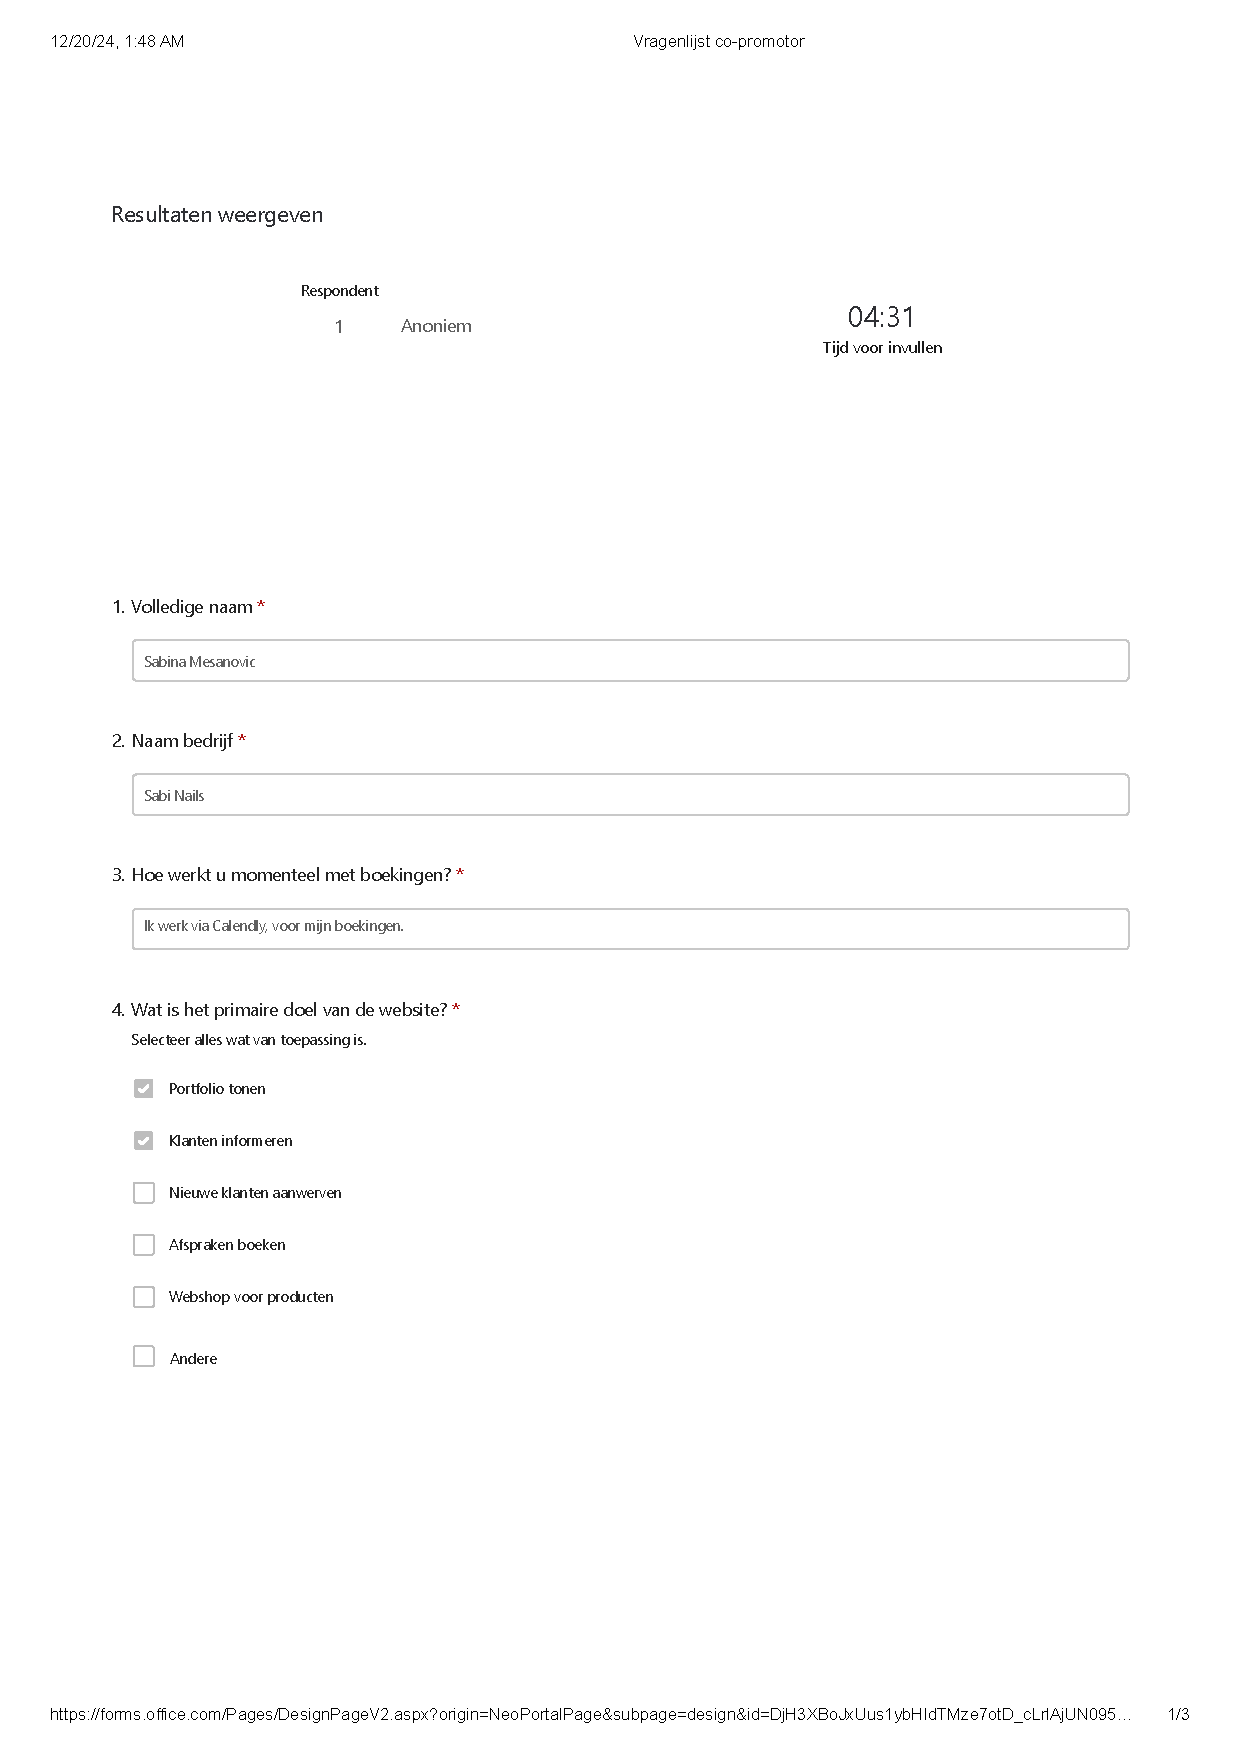
\includepdf[pages=-,alt={'Vragenlijst co-promotor'}]{./Vragenlijst_co-promotor.pdf}

\end{document}